% Build from this directory with latexmk -pdf report.tex.
\documentclass[11pt,letterpaper]{article}

\usepackage[T1]{fontenc}
\usepackage{newtxtext,newtxmath}
\usepackage[margin=0.78in,bottom=0.72in]{geometry}
\usepackage{graphicx}
\usepackage{booktabs,tabularx}
\usepackage{caption}
\usepackage{float,titlesec}
\usepackage[authoryear,square]{natbib}
\usepackage[colorlinks=true,citecolor=blue,linkcolor=blue,urlcolor=blue]{hyperref}

\linespread{0.94}
\raggedbottom
\titlespacing*{\section}{0pt}{13pt}{6pt}
\titlespacing*{\subsection}{0pt}{8pt}{4pt}
\setlength{\intextsep}{8pt plus 2pt minus 2pt}
\setlength{\parindent}{0pt}
\setlength{\parskip}{4pt plus 1pt minus 1pt}
\setlength{\bibsep}{3pt}
\setcounter{secnumdepth}{3}
\captionsetup{font=small,skip=5pt,labelsep=period,justification=justified,singlelinecheck=false}
\newcolumntype{Y}{>{\centering\arraybackslash}X}
\newcolumntype{L}[1]{>{\raggedright\arraybackslash}p{#1}}

\ifdefined\pdfinterwordspaceon
  \pdfinterwordspaceon
\fi

\begin{document}

\begin{center}
{\Large\bfseries Optimal Block Size Prediction Through Least Size Kernel Representation\par}
\vspace{4pt}
[Author names]\\
New York University, [course and term]\\
{\small\texttt{[NYU email addresses]}}
\end{center}

\begin{abstract}
While choosing the correct CUDA block size for launching a kernel is important, the tool doing the same in runtime itself might incur significant delay. The existing methods generally reduce the kernel to a fixed size vector representation, and then find the optimal block size through a lightweight neural-network. We update this architecture by allowing the system to choose a variable size kernel representation. During training, the model learns to find the shortest kernel representation that preserves block-size prediction quality, thereby minimizing the runtime overhead of the lightweight selector. Our model learns gates over LSTM states, caches the surviving states at build time, and uses workload dimensions to score candidate sizes at runtime. On 2,785 held-out LS-CAT cases, adaptive retention pruned 16.7\% of optional gates and
achieved 5.54\% mean runtime regret at its selected epoch, compared with 5.48\% for the full-sequence model.
Across 13 live cases, toolcall achieved 1.05--1.50\ensuremath{\times} speedup over fixed 256-thread blocks
with selection time included.
\end{abstract}

\section{Introduction}

A CUDA launch divides work into a grid of thread blocks. A GPU schedules blocks onto streaming
multiprocessors (SMs), where threads execute in warps of 32. For a one-thread-per-item kernel processing
1,000 elements, a 256-thread block requires four blocks and an index check in the last one. A 64-thread
block requires 16 blocks and the same kind of check. Both launches cover the same elements, but they change
the number of blocks the GPU can distribute and the resources allocated to each block.

The useful configuration depends on how the kernel performs its work. More resident warps can help hide
latency. Registers and shared memory can limit residency, and the block shape can affect data reuse, memory
access patterns, and the amount of inactive work near input boundaries. A sweep measures the net effect for
a specific workload, but a production launch may have only one chance to make the decision.

We study a selector that chooses among 16 thread counts from 64 through 1024 in steps of 64. The application
determines the grid that covers its work. Throughout the report, the fastest measured candidate means the
valid tested configuration with the lowest measured time for a specified kernel, input, device, and timing
protocol.

The LS-CAT dataset and its companion predictor showed that LLVM IR contains information about efficient
launch choices \citep{bjertnes2021a,bjertnes2021b}. We started with that separation of code and
workload inputs and examined where to reduce the cost of a prediction. An LSTM can summarize the entire
kernel in its final state, but that single vector may hide details available at intermediate positions.
Keeping every state exposes those details and requires scoring work proportional to the number of states. We
test whether the model can learn a smaller, kernel-specific representation that still chooses a fast
configuration.

We follow this question from the 12-kernel pilot to a larger source-group-held-out LS-CAT experiment and
then to a CUDA launch that includes measured CPU selection time. The deployment test matters because even a
good block prediction only saves time when the faster GPU launch repays the cost of making it.

\section{Literature Survey}

\subsection{Architecture guided and static tuning}

Architecture-guided tuning explains performance using the resources a kernel consumes. Dense linear algebra
experiments showed that register blocking and instruction-level parallelism can yield high performance at
lower occupancy \citep{volkov2008}. This gives a reason to treat occupancy as one factor in launch
selection. A static CUDA autotuner combines program analysis and GPU characteristics to select parameters
without running each configuration \citep{lim2017}. Static approaches avoid per-case measurement when their
models capture the relevant bottlenecks. The assumptions in those models determine how well the
recommendations transfer.

\subsection{Measurement based autotuning}

Empirical autotuners run candidate implementations and search for the fastest measured configuration. Kernel
Tuner \citep{vanwerkhoven2019} searches parameterized GPU kernels and can tune block dimensions jointly with
choices such as tiling or unrolling. Measuring on the target workload captures interactions that a simple
analytic model can miss. The evaluation cost grows as the candidate space expands, and a new input or device
can require another search. In this project, sweeps serve as training data and reference measurements. The
deployed selector makes its decision with one model evaluation.

\subsection{Learning from program representations}

Learned tuning replaces some search with predictions from previous measurements. A study of OpenCL stencils
compared classifiers and performance regressors for workgroup-size prediction \citep{cummins2016}. The
comparison illustrates why runtime loss matters when several configurations have similar performance. LS-CAT
supplies measured runtimes for CUDA kernels collected from public repositories \citep{bjertnes2021a}. A
follow-up study used LLVM IR token sequences and learned embeddings to predict launch choices from this
corpus \citep{bjertnes2021b}. The approach can make a prediction for an unmeasured workload, and its
reliability depends on representative training data and separation of related source code during evaluation.

The LS-CAT prediction study motivates the code encoder in this project. We extend that design by comparing a
workload-only model with full and selectively retained code representations, then embedding a trained
selector in a CUDA host program. This lets us ask whether the code representation earns its runtime cost, a
question that an offline score alone cannot answer.

\section{Proposed Idea}

\subsection{The baseline published predictor and our new proposed solution}

We use the NLP-based block-size predictor proposed by \citep{bjertnes2021b} as our baseline, referring to it throughout this report as the original LS-CAT predictor. In the original LS-CAT predictor, the CUDA kernel’s LLVM IR is encoded using frozen FastText embeddings and then processed by an LSTM. The authors also evaluated an LSTM-based architecture with attention. The transformed recurrent representation is combined with a learned embedding identifying the LS-CAT workload (like encoded input size) instance before being passed to the dense prediction layers. Dense layers then predict a value for each
block size. We retained the use of IR, a recurrent encoder, and a the last stage dense-layer with attention based prediction, but allow the dense-layer to take input of variable lengths. In the following subsections, we discuss in detail each of the concerned modules involved. 

\begin{figure}[H]
\centering
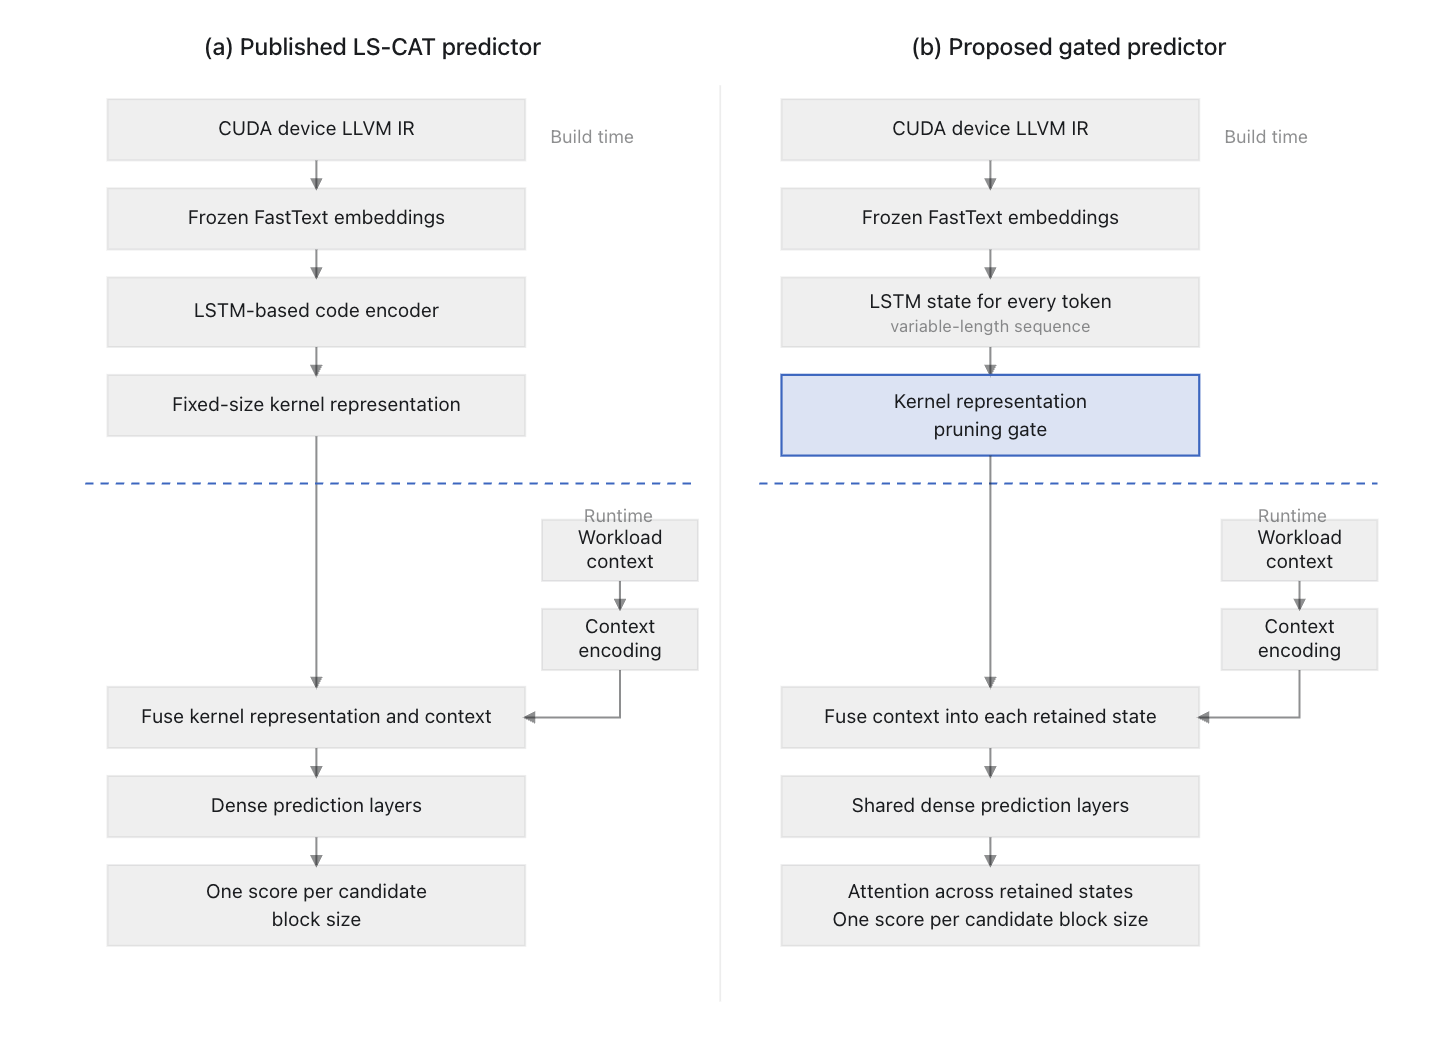
\includegraphics[width=.84\linewidth]{figures/architectures_2.png}
\caption{The published LS-CAT predictor, redrawn from Figure 1 of \citep{bjertnes2021b}, and the proposed gated
predictor. The dashed line marks the handoff from the cached code representation to runtime scoring.}
\label{fig:architectures}
\end{figure}


\subsection{Kernel Preprocessing Phase in Compilation}
Here we discuss the components: CUDA LLVM IR, Frozen FastText Embedding and LSTM based encoder that are run during compile time.

Clang produces LLVM IR (Internal Representation) for the kernel code. The frontend tokenizes the IR and maps tokens to frozen
40-dimensional FastText vectors \citep{bojanowski2017}. An LSTM \citep{hochreiter1997} then reads every embedded
token in order and produces one state ($h_i$) per token. Now, each state $hi$ is produced taken the $1 - ith$ token under consideration.
Hence, as we go from $h1$ to $h_N$, we get a summarization of a larger portion of the kernel logic. This follows that 
the final state $h_N$ contains a compact summarization of the whole kernel. As the summarization becomes increasingly comapct, we might lose 
important information along the way. Hence, we consider using a subset of states from $h1$ to $h_{N - 1}$ using a Pruning Gate, as discussed later, for making the prediction.


\subsection{Kernel Representation Pruning Gate}
Here we discuss the Pruning Gates that select the subset of states generated by LSTM to be considered for the final prediction. The gate for a position reads that position's state
together with the final LSTM state. This pairing lets a gate compare a local summary with a summary of the
full kernel. The final state is always retained, so even the most compressed representation contains a state
that has read the full input.

The Pruning Gates use the hard-concrete construction \citep{louizos2018}. Training samples continuous gate
values with a probability of exactly zero and adds a penalty proportional to the expected number of open
states (more of it in Training Loss subsection). Evaluation uses deterministic gate values. It removes zero-gated rows and caches the surviving
hidden states and gate values. Gate selection depends on the kernel code, so the representation can be
reused across input dimensions. Every token is still encoded at build time. Closing gates saves storage and
reduces the number of rows scored at runtime.

\subsection{Fusing Kernel Context and Workload Encoding}
This component, unlike the proceeding components, is run at runtime. This phase consists of WorkLoad encoder, Shared Dense Prediction Layer and Attention based weighted sum.

The WorkLoad encoder takes in the problem size $(m, n)$ a list of 2 elements. For problems requiring only one dimensional input (example vector addition with same length vector), the problem size can be put as (m, 1).
The workload encoder log-scales the dimensions and projects them into 32 features. We concatenate that
context with every retained state from the Pruning Gates and run the same dense layers on each row, with hidden sizes of 256, 128,
and 64. Each row produces 16 block-size logits and a scalar attention score. The model multiplies the
attention weights by the gate values and renormalizes across the retained rows as follows:
\[

Score_{16} = \sum_{i = 1}^{K} w_i * F(h_i) ~~\text{Where F(h_i) is the dense layer output for $i$th kernel represtation, K is the total number of gates retained.}
\]

The weighted sum yields one logit per block size. Workload-dependent attention can emphasize different parts of the same cached
representation at different input sizes. The system learns its own retention count.


\subsection{Training Loss}
Here we define the losses used for training the system. We start with Baseline experiment with a simple Mean Square Error between 
the Fastest measured runtime and the Runtime of predicted configuration. In this first experiment, we do not consider penalizing the model
for considering the full representation of the Kernel. So we get the loss $L$ as
\[
L = L_{MSE}
\]

We then further update this to penalize the length of the kernel considered for the prediction. This encourages the model
to make a good prediction considering the minimum amount of kernel information. Given that the number of operations (and hence the time to run) for the Dense Layer + Attention component
of our system is directly proportional to the number of kernel representation inputs considred, this helps produces a good predictor that itself takes minimal amount of time.
This new loss term $L_{length}$ is defined as the expected number of gates open. In other words:
\[
L_{length} = \sum_{i=1}^{K - 1} P(i) ~~ \text{Where P(i) shows the probability of the Pruning Gate being open.}
\]
The full loss function stands as:
\[
L = L_{MSE} + \lambda_1 L_{length}
\]

In the third experiment, we try to reduce the amount of instability in the model, as it is observed during the training with the previous
loss function. Here, we add a KL divergence term to restrict the movement of the model in order to increase the stability of training.
We get
\[
L = L_{MSE} + \lambda_1 L_{length} + \lambda_2 L_{KL,ema_decay=0.99,temp=2.0}
\]


\subsection{Compiling and launching a user kernel}
In this part, we provide an argonomic easy-to-use tool to compile and use our thread count predictor.
To use the selector, include \texttt{toolcall.hpp} in the CUDA host code and call \texttt{model\_output}
with the kernel and workload. The API returns the grid and block dimensions for one-dimensional coverage. It is important to note that
our system just predicts the block size as of now. We provide the block count by finding (problem size / block size). The user is in 
liberty to use this block count, or use their own function that finds block count using our predicted block size if it is critical for correctness.
The scorer masks unsupported candidates using device and kernel launch limits. The wrapper accepts explicit
\texttt{work\_items} so launch coverage follows the indexing of the kernel, while m, n, and k provide the
model's workload features.

\begin{verbatim}
#include "toolcall.hpp"
auto [grid, block] = toolcall::model_output(my_kernel, {m, n, k, work_items});
my_kernel<<<grid, block>>>(device_args);
\end{verbatim}

Build the executable with \texttt{./toolcall my\_kernel.cu -o my\_program}. The wrapper extracts the
kernel's LLVM IR, runs the encoder and gates, and includes the cached representation in the launch
artifacts. Softmax uses one thread per vector, so its grid rounds up the vector count. ComputeOrientations
assigns a warp to each keypoint. Matrix multiply + ReLU uses 32 columns per block tile and derives the tile
height and grid from the predicted thread count.

\subsection{Native and compiled CPU scorers}

As loading and running the tool adds to the total overhead, we explore a native and a compiled method for the same. The native path implements the context encoder, dense layers, and attention directly in C++ with weights
generated from the checkpoint. With \texttt{--aot}, PyTorch's AOTInductor exports and compiles the same CPU
scoring graph and packages its trained weights. The CUDA host program loads the compiled package through
LibTorch. Both backends use the same \texttt{model\_output} API and run the user's kernel on the GPU. The
compiled path specializes the scoring graph for the cached state count, which is known when the program is
built.

\section{Experimental Setup}

\begin{table}[H]
\centering\small
\caption{Devices and software used for the recorded experiments.}
\begin{tabularx}{\linewidth}{@{}L{.19\linewidth}L{.32\linewidth}>{\raggedright\arraybackslash}X@{}}
\toprule
\textbf{Experiment} & \textbf{Device} & \textbf{Recorded software or source} \\
\midrule
Local 1D sweeps & RTX 2080 Ti \textbullet{} 68 SMs \textbullet{} CC 7.5\newline A100-SXM4-40GB \textbullet{} 108 SMs \textbullet{} CC 8.0 & Linux and NVCC 13.0.88. Device and environment logs are stored with each run. \\
LS-CAT model comparison & NVIDIA T4 for archived labels\newline NVIDIA TITAN V in model timing logs & PyTorch 2.8.0+cu128 and CUDA 12.8 in the model logs. Clang/LLVM and FastText for the frontend. \\
Live launch benchmarks & CPU scorer and CUDA GPU execution & C++17/CUDA benchmark sources and toolcall build wrapper. \\
\bottomrule
\end{tabularx}
\end{table}

\subsection{Model validation on the public CUDA corpus}

We import the full available one-dimensional set from the public LS-CAT T4 archive.
As we are only considring 16 candidate 1D thread counts, the import script, \texttt{scripts/import\_lscat.py}, only keeps those 16-candidate cases, averages duplicate
archived timings, and drops invalid timings. The frontend and FastText scripts prepare token IDs and
matching frozen embeddings. The saved split contains 400 source groups for training (2,050 kernels, 16,423
cases) and 50 groups for validation (338 kernels, 2,785 cases). The same source group stays on one side of
the split.

Recreate the saved comparison with \texttt{scripts/train\_adaptive.py} and the split stored in the
checkpoint. Use model and split seed 2, 120 epochs, batch size 8, AdamW at 0.001, zero weight decay,
gradient clipping at 1, and BCE targets with exponent 12. The sequence models use LSTM width 1. The adaptive
runs use a length penalty of \(10^{-8}\) with KL weights of 0 and \(10^{-4}\). For the KL run, the
temperature is 2 and the teacher decay is 0.99. Checkpoints are selected by validation regret, then task
loss.

\subsection{Live timing protocol}
Here we share the timing protocol used for a kernel using a trained frozen model. We first build the fixed and toolcall variants from \texttt{examples/runtime\_launch} and pass the inputs and block
sizes. We Use \texttt{scripts/collect\_launch\_benchmarks.py} to collect
results. After five warm-ups, the benchmark records medians over 51 trials for CPU selection time, GPU time,
and host time from selection to synchronized kernel completion. The GPU event timer uses a separate launch.
The reported host interval begins after buffer setup and ends before output verification. We run this test expriment on softmax, ReLU, Orientation kernels.


\subsection{Selection of Kernels with pruning}
We further analyze what kind of kernels are getting higher prunings and which ones are not. We see that it is the bigger kernels like ComputeOrientations, Find3DMinMax, mat_mul_shared that are getting higher 
amount of pruning. More formally, kernels producing $>1200$ representation tokens were more likely to get pruning rest of the ones. There are no kernels
with representation token count $<1000$ that experienced pruning. We further quantify the reuslt for some of the test kernels in the following table [citation required].

\begin{table}[H]
\centering\small
\caption{LS-CAT results at each model's best-validation-regret epoch.}
\begin{tabularx}{\linewidth}{@{}L{.24\linewidth}YYYYY@{}}
\toprule
\textbf{Kernel} & \textbf{Kernel Representation Size} & \textbf{Retained} & \textbf{percentage pruning} \\
\midrule
ComputeOrientations & 12,955 & 2,280 & 82.40\% \\
Find3DMinMax & 3,305 & 1,203 & 63.60\% \\
mat_mul_shared & 2,286 & 1,185 & 83.3\% \\
matrixMultiplyAndSigmoid & 2,574 & 1,341 & 48.16\% \\
gpu_blur & 1,855 & 1,015 & 45.28\% \\
\bottomrule
\end{tabularx}
\end{table}

\section{Experiments \& Analysis}

\subsection{Measures of success}

We primarily measure performance for comparision purposes. We define performance as follows:

\[
Performance = \frac{\text{Fastest measured runtime}}{\text{Runtime of predicted configuration}}
\]

Performance compresses the results into [0,1] interval. Given that we count time in microsecond granularity and kernels can take upto seconds to run full, this causes the reults to be clustered around $0.95$. Recognizing that
we measure performance accurate upto $0.0001$ given an improvment of that level in performance may still be significant.

For deployment, speedup is the fixed-run median host time divided by the model-run median host time. A value above one means the GPU time
saved was sufficient to cover selection for the recorded workload. Retained-state fraction measures how much
of the original sequence the scorer must process.


\subsection{Validation performance and retained states}

\begin{table}[H]
\centering\small
\caption{LS-CAT results at each model's best-validation-regret epoch.}
\begin{tabularx}{\linewidth}{@{}L{.24\linewidth}YYYYY@{}}
\toprule
\textbf{Model} & \textbf{Epoch} & \textbf{Performance score} & \textbf{Optional states kept} \\
\midrule
Context only & 78 & 0.9508 & 0\% \\
Full sequence & 50 & 0.9519 & 100.0\% \\
Adaptive without KL & 41 & 0.9517 & 83.3\% \\
Adaptive with KL & 31 & 0.9512 & 100.0\% \\
\bottomrule
\end{tabularx}
\end{table}

Here, in case of context only expriment, we keep all the gates closed and cut-off the information of the kernel. This follows a validation curve without much impromvement, showing kernel information is important for finding pattern in the optimal thread counts.
We then try full retention to show that using full kernel information, we can indeed achieve a decreasing validation curve and increase in performance. Using full sequence achieved the highest performance on the validation split.
Finally our proposed adpative model without KL acheived a performance of around 0.9517, in the range of 0.0002 percent with the full sequence. The important observation here is that
this performance was achieved even after pruning $16.7\%$ of the kernel representation on an average, hence lowering the prediction time of the tool.
We also experiment with a KL divergence term in our loss functin. We observe that upon introducing a KL divergence term, the model prefers less pruning. Hence, when it achieves highest performance
we get no pruning. Given the maximum performance by non kl training both exceeds that of with a KL term and achieves consistent pruning, we conclude that the non-kl based loss function is the optimal choice for us.
Other than that, we observe exact-winner accuracy to fall for both of non-kl and kl based approaches. Here, consider exact-winner accuracy as just the raw classification accuracy, considering all 16 thread counts as indendent classes.

\subsection{Effect of KL regularization: Why it did not improve performance}

We use Kullback--Leibler (KL) divergence to encourage the current model to match the candidate score
distribution of a teacher formed by an exponential moving average of earlier weights. The intent is to
stabilize predictions as the gates change. At their selected epochs, the no-KL run had slightly higher performance
(0.9517\% versus 0.9512\%) and pruned more optional states (16.7\% versus 0\%). One explanation is that matching
an earlier distribution makes it harder for the scorer and gates to adjust together as states close. The
saved runs support the trade-off at the selected checkpoints. Establishing that mechanism would require
repeated matched runs.

At epoch 120 the no-KL run pruned 38.8\% of optional states, and performance decreased to 0.9471\%. The KL run pruned
4.5\% and recorded a higher performance than its non-kl version. This illustrates why the best checkpoint for deployment may
differ from the one with the smallest representation. A small loss in block selection quality can be
worthwhile if processing fewer rows saves more time than the selected block loses on the GPU. We measure
the two costs together at launch.

\subsection{Live launch performance}

\begin{table}[H]
\centering\small
\caption{Deployment results using host time from selection through completion. Pruning is the percentage of pre-gate kernel states removed.}
\begin{tabularx}{\linewidth}{@{}L{.20\linewidth}cYYYYY@{}}
\toprule
\textbf{Benchmark} & \textbf{Cases} & \textbf{Model threads} & \textbf{Best fixed threads} & \textbf{Speedup vs. 256} & \textbf{Gap to best fixed} & \textbf{Pruned states} \\
\midrule
Softmax & 4 & 576 & 544/576 & 1.41--1.50\ensuremath{\times} & 0.49--9.36\% & 0.00\% \\
Matrix multiply + ReLU & 4 & 512 & 1024 & 1.20--1.21\ensuremath{\times} & 0.70--1.01\% & 63.52\% \\
ComputeOrientations & 5 & 64 & 64 & \ensuremath{\approx}1.055\ensuremath{\times} & 0.16--0.33\% & 81.38\% \\
\bottomrule
\end{tabularx}
\end{table}

\begin{figure}[H]
\centering
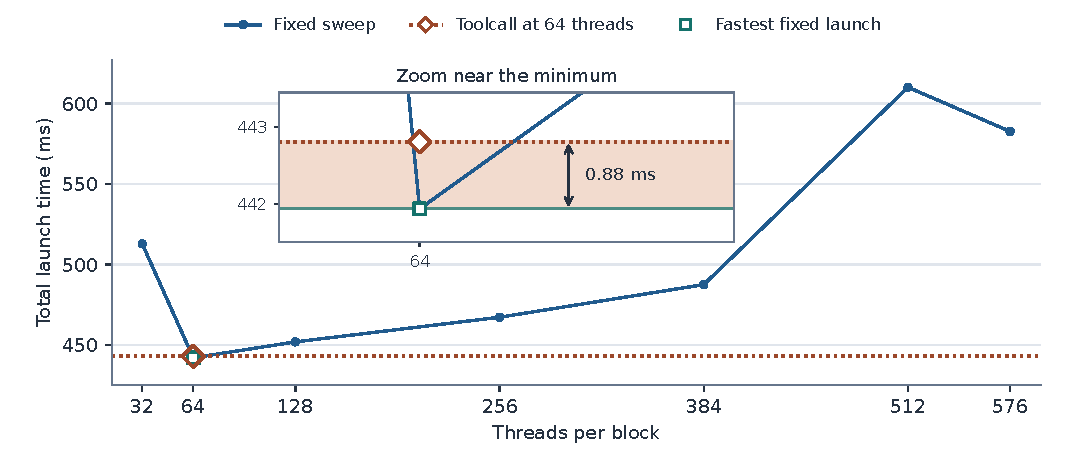
\includegraphics[width=.94\linewidth]{figures/compute_orientations_single.pdf}
\caption{ComputeOrientations with 64,194,304 keypoints on a \(4{,}096\times4{,}096\) image. The dotted line
shows Toolcall's total time at 64 threads (442.81 ms). The fixed sweep also reaches its minimum at
64 threads (441.93 ms). The shaded 0.88 ms gap is what we aim to minimize, bringing Toolcall's total time,
including selection, closer to the fastest measured fixed launch.}
\label{fig:orientations-single}
\end{figure}

\begin{figure}[H]
\centering
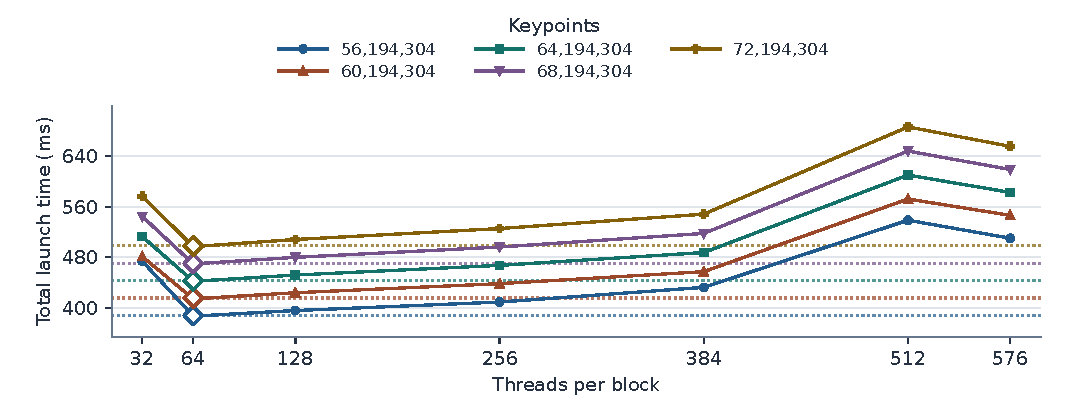
\includegraphics[width=.94\linewidth]{figures/compute_orientations_sweep.pdf}
\caption{ComputeOrientations for all five measured keypoint counts on a \(4{,}096\times4{,}096\) image.
Solid curves connect fixed-block measurements. Each matching dotted line shows Toolcall's total time,
with a diamond at its predicted block size.}
\label{fig:orientations-sweep}
\end{figure}

\begin{figure}[H]
\centering
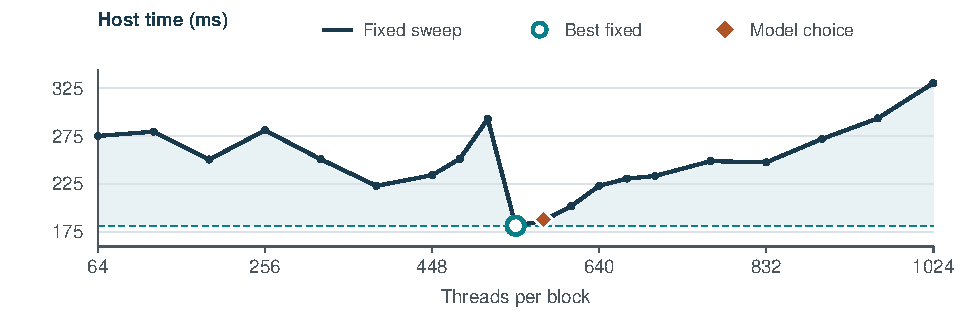
\includegraphics[width=.92\linewidth]{figures/softmax.pdf}
\caption{Softmax for all four measured problem sizes, shown as the number of vectors and their length.
Solid curves connect fixed-block measurements. Each matching dotted line shows Toolcall's total time,
with a diamond at its predicted block size.}
\label{fig:softmax}
\end{figure}

For the 150,051-vector input of length 1,500 in Figure~\ref{fig:softmax}, the model took 187.85 ms compared with 281.19 ms at fixed
256 and 181.52 ms at fixed 544. At fixed 576, the same block chosen by the model took 186.68 ms. The
same-block comparison shows a 1.17 ms difference in total time, close to the separately recorded 1.16 ms
selection time. The 256-thread block had enough headroom for the prediction to pay off. The 544-thread fixed
candidate kept a smaller advantage over the model.

\begin{figure}[H]
\centering
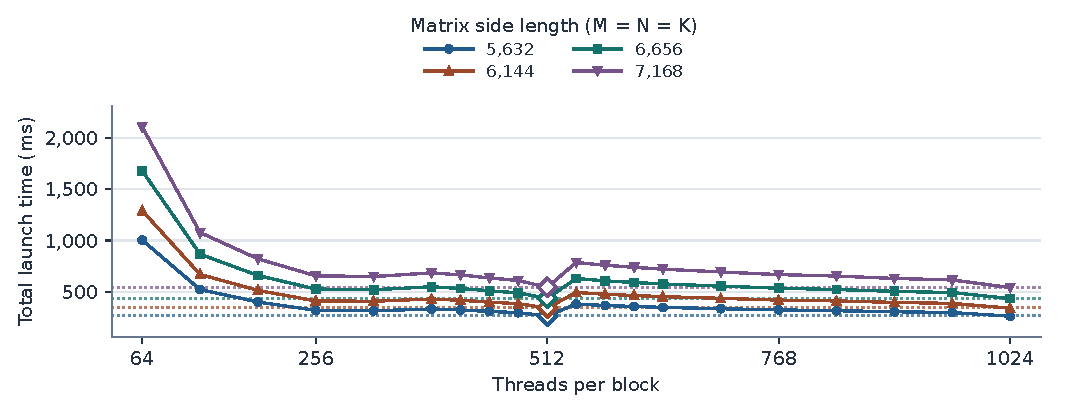
\includegraphics[width=.94\linewidth]{figures/matrix_relu_sweep.pdf}
\caption{Matrix multiply + ReLU for all four measured square problem sizes. Solid curves connect fixed-block
measurements. Each matching dotted line shows Toolcall's total time, with a diamond at its predicted block size.}
\label{fig:relu-sweep}
\end{figure}

For matrix multiply + ReLU, the model's 512-thread choice had a total-time gap of 0.70--1.01\% from the
fastest measured fixed launch (Figure~\ref{fig:relu-sweep}). A 512-thread block covers 16 rows per tile and
a 1024-thread block covers 32. Changing rows per tile changes the work per block and shared memory usage.
For ComputeOrientations, the model chose the same block size as the best fixed run on every input
(Figure~\ref{fig:orientations-sweep}). Each warp has its own scratch space, so larger blocks request
more shared memory. Profiling would be needed to distinguish residency, reuse, and scheduling effects. The
model saved time against fixed 256 in both workloads.

The deployed checkpoint retained 3,165 of 3,165 states on softmax, 1,301 of 3,566 on matrix multiply + ReLU,
and 2,076 of 11,149 on ComputeOrientations. Measured selection medians across the three kernels ranged from
1.06 to 1.46 ms. The cases differ in code, input, and kernel duration. A matched run using alternate
retention counts for the same kernel would be needed to measure the effect of pruning on selection time.

\subsection{Scorer backend comparison}

In the development tests, we observed substantially faster CPU scoring with the AOTInductor package
than with the native C++ implementation. A plausible contributor is that AOTInductor compiles the scoring
graph into optimized CPU code specialized for the cached state dimensions. The archived launch sweeps lack
matched native and AOT rows with recorded backend and build settings, so we report the direction observed in
development and leave its speedup unquantified.


\subsection{When to use the selector}

The break-even test is whether the GPU time saved over the current fixed block exceeds the extra CPU
selection time. Large workloads are good candidates when the difference between the baseline block and a
fast block grows in absolute time. In the softmax example, total time fell by 93.34 ms against fixed 256,
while a same-block comparison put the added cost at about 1.17 ms. The available gain is specific to the
workload and reference block. Hence, we recommend to use the proposed system when the kernel runtime is atleast of the order of seconds, such that 
added cost of our tool (average about 1-2ms sensitive to h size) is a non-issue. So sensitive to kernel size, the system useful 
as the problem size increases.

To better understand the effect of problem size, we draw the block-size versus runtime plots [citeation required]. Here, we do a sweep of multiple 
block sizes, making one curve for each prolem size. We then draw a horizontal line for each problem size that shows the time required by our
proposed system. We then observe the area between the curve and the horizontal line. The excess area above the measured minimum describes how sensitive
the sweep is to block choice. A small area after normalizing for the minimum runtime means many blocks are
close to the best in relative terms. It makes a slightly imperfect prediction less costly, while also
leaving less tuning headroom when the fixed baseline lies in the same flat region. A higher area would mean the total time taken by the tool and the kernel
ran on the proposed block size is higher than more of the optimal block sizes ran without our tool.

\section{Conclusions}
Here we successfully develop a system that considers a minimal set of the kernel representation to predict optimal block size, making it faster than its contemporary systems that takes a fixed block count.
    
We also see that kernels with bigger representations actually have more redundant information for optimal block count prediction, hence allowing scope of more pruning.

\begin{thebibliography}{9}
\small

\bibitem[Bjertnes et al.(2021a)]{bjertnes2021a}
Lars Bjertnes, Jacob O. Tørring, and Anne C. Elster, ``LS-CAT: A Large-Scale CUDA AutoTuning Dataset,'' in
IEEE International Conference on Applied Artificial Intelligence (ICAPAI), 2021a.

\bibitem[Bjertnes et al.(2021b)]{bjertnes2021b}
Lars Bjertnes, Jacob O. Tørring, and Anne C. Elster, ``Autotuning CUDA: Applying NLP Techniques to LS-CAT,''
in Norsk informatikkonferanse (NIKT), pp. 72--85, 2021b.

\bibitem[Bojanowski et al.(2017)]{bojanowski2017}
Piotr Bojanowski, Edouard Grave, Armand Joulin, and Tomas Mikolov, ``Enriching Word Vectors with Subword
Information,'' Transactions of the Association for Computational Linguistics, vol. 5, pp. 135--146, 2017.

\bibitem[Cummins et al.(2016)]{cummins2016}
Chris Cummins, Pavlos Petoumenos, Michel Steuwer, and Hugh Leather, ``Autotuning OpenCL Workgroup Size for
Stencil Patterns,'' in 6th International Workshop on Adaptive Self-Tuning Computing Systems, 2016.

\bibitem[Hochreiter and Schmidhuber(1997)]{hochreiter1997}
Sepp Hochreiter and Jürgen Schmidhuber, ``Long Short-Term Memory,'' Neural Computation, vol. 9, no. 8, pp.
1735--1780, 1997.

\bibitem[Lim et al.(2017)]{lim2017}
Robert V. Lim, Boyana Norris, and Allen D. Malony, ``Autotuning GPU Kernels via Static and Predictive
Analysis,'' in 46th International Conference on Parallel Processing (ICPP), pp. 523--532, 2017.

\bibitem[Louizos et al.(2018)]{louizos2018}
Christos Louizos, Max Welling, and Diederik P. Kingma, ``Learning Sparse Neural Networks through \(L_0\)
Regularization,'' in 6th International Conference on Learning Representations (ICLR), 2018.

\bibitem[van Werkhoven(2019)]{vanwerkhoven2019}
Ben van Werkhoven, ``Kernel Tuner: A Search-Optimizing GPU Code Auto-Tuner,'' Future Generation Computer
Systems, vol. 90, pp. 347--358, 2019.

\bibitem[Volkov and Demmel(2008)]{volkov2008}
Vasily Volkov and James W. Demmel, ``Benchmarking GPUs to Tune Dense Linear Algebra,'' in Proceedings of the
ACM/IEEE Conference on Supercomputing (SC), 2008.

\end{thebibliography}

\end{document}
